\documentclass[11pt,a4paper]{book}
\usepackage[utf8]{inputenc}
\usepackage[spanish,es-tabla]{babel}
\usepackage{amsmath}
\usepackage{amsfonts}
\usepackage{amssymb}
\usepackage{graphicx}

\usepackage{vmargin}

\usepackage{hyperref}

\setpapersize{A4}
\setmargins{2.5cm}       % margen izquierdo
{1.5cm}                        % margen superior
{16.5cm}                      % anchura del texto
{23.42cm}                    % altura del texto
{10pt}                           % altura de los encabezados
{1cm}                           % espacio entre el texto y los encabezados
{0pt}                             % altura del pie de página
{2cm}                           % espacio entre el texto y el pie de página

\title{Notas del curso socket.io}
\author{Saez, Lautaro Andres}
\date{\today}


\begin{document}
    \maketitle


    \chapter{Aprendiendo Socket.io}

    \section{WebSockets}

    Es una tecnología que hace posible establecer una conexión full-duplex, 
    entre un cliente y servidor.

    \section{Comunicación}

    La comunicación a través de un servidor nunca entre clientes.

    \section{Primer socket server}

    \subsection{Configuracion}

    Debemos iniciar un projecto de Node con el comando \textit{npm init}. Luego 
    necesitamos instalar:

    \begin{itemize}
        \item socket.io 
        \item express
    \end{itemize}

    \subsection{Nociones basicas}

    Al importar el módulo socket.io es necesario crear una instancia de dicho módulo, a la cual le debemos pasar el server de express, como se 
    muestra en la Figura \ref{fig:socket-create}.
    
    \begin{figure}
        \centering
        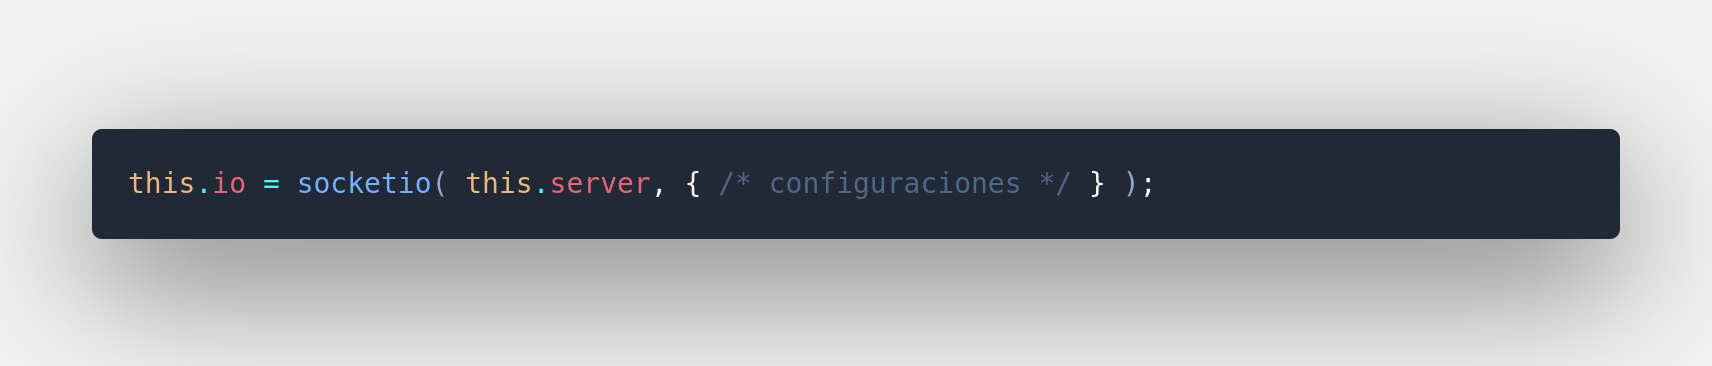
\includegraphics[width=.8\textwidth]{img/socket-create.png}
        \caption{Creación del socket.}
        \label{fig:socket-create}
    \end{figure}

    \subsection{Estableciendo una conexión}

    Para establecer una conexión debemos utilizar el método $on$ del objeto io, escuchando el socket \textit{connection}. 
    Otro argumento de método $on$ es una callback function, la cual indica que las acciones que vamos a utilizar 
    durante la conexion, esta función recibe un parámetro el que hace referencía al socket del cliente.

    \subsection{Métodos basicos} 

    Tanto el objeto io, como el client tienen 2 funciones basicas: 

    \begin{itemize}
        \item on: recibe el nombre del socket para escuchar, y una callback function que recibe la data.
        \item emit: recibe el nombre del socket a escuchar, y la data a enviar (usualmente un JSON).
    \end{itemize}

    

\end{document}